\documentclass[10pt,twoside]{article}

% !TEX program = xelatex
% ==================== NeurIPS 样式（预印本版式）====================
\usepackage[preprint]{neurips_2025}
\geometry{marginparwidth=0.4in, marginparsep=0.1in}

% ==================== 中文支持（XeLaTeX + ctex）====================
\usepackage[UTF8]{ctex}

% ==================== 数学与符号 ====================
\usepackage{amsmath,amssymb,amsfonts,amsthm}
\usepackage{mathtools}
\usepackage{bm}
\usepackage{siunitx}

% ==================== 图表 ====================
\usepackage{graphicx}
\usepackage{xcolor}
\usepackage{booktabs}
\usepackage{multirow}
\usepackage{array}
\usepackage{tikz}
\usetikzlibrary{arrows.meta,positioning,calc,fit,shapes.geometric}
\usepackage{caption}
\usepackage{subcaption}

% ==================== 浮标布局 ====================
\usepackage[section]{placeins}
\renewcommand{\topfraction}{0.92}
\renewcommand{\bottomfraction}{0.85}
\renewcommand{\textfraction}{0.06}
\renewcommand{\floatpagefraction}{0.72}

% ==================== 链接与引用 ====================
\usepackage[colorlinks=true, linkcolor=black, citecolor=black, urlcolor=black]{hyperref}
\usepackage{url}
\usepackage{enumitem}

% ==================== 自定义命令 ====================
\newcommand{\stopgrad}{\operatorname{sg}}
\newcommand{\topk}{\operatorname{TopK}}
\newcommand{\softmax}{\operatorname{softmax}}
\newcommand{\softplus}{\operatorname{softplus}}
\newcommand{\sigmoid}{\operatorname{sigmoid}}
\newcommand{\R}{\mathbb{R}}
\newcommand{\E}{\mathbb{E}}

% ==================== 定理环境 ====================
\theoremstyle{definition}
\newtheorem{definition}{定义}[section]
\newtheorem{assumption}{假设}[section]
\theoremstyle{plain}
\newtheorem{theorem}{定理}[section]
\newtheorem{lemma}{引理}[section]
\newtheorem{corollary}{推论}[section]
\newtheorem{proposition}{命题}[section]
\theoremstyle{remark}
\newtheorem{remark}{注}[section]

% ==================== 元信息 ====================
\title{重构冻结的异构预训练模型：\\ 子层融合、协调式路由与嵌合蒸馏}

\author{
    匿名作者\\
    单位\\
    \texttt{email@example.com}
}

\begin{document}

\maketitle

\begin{abstract}
将异构预训练模型——双向编码器、因果解码器与视觉 Transformer，它们在架构、隐藏宽度与模态上各不相同——组合起来，通常需要联合重训练、架构手术或有损的输出层集成。本文研究如何在所有底座保持冻结的前提下，分三步\emph{重构}这类模型。\textbf{（i）子层融合。}一个共享的稀疏 Top-$K$ 路由器为每个 token 在 $M$ 个冻结的架构专家中选择其一；语义对齐器把互不匹配的隐藏空间映射进同一路由空间；专家经逐专家门控做残差融合。在四种对齐器设计上，我们测得一条严格但\emph{饱和}的阶梯（线性 $<$ 均值 $<$ 跨架构注意力 $<$ mixture），且容量匹配对照表明这一天花板来自设计而非参数量。\textbf{（ii）协调式路由。}我们追问一个全局中枢应当如何影响共享路由器，并证明在四种中枢模式中，只有调制 Softmax 温度（门控式）同时满足完美退化、保序、有界与低开销；我们还诊断出一个隐藏失效模式——长训练中 tanh 饱和切断了通往中枢的梯度。\textbf{（iii）独立模型重构。}嵌合蒸馏把集成坍缩为单底座学生，而对损失中直接目标项权重的连续扫描表明，表观的``学生优于教师''裕度全部归因于该目标项，而非概念方向传递或方差平均。由于融合推理要求每个底座存活、蒸馏又是部署手段，这项研究的可信度完全取决于其评估方式。因此我们在全栈统一施加\emph{样本外纪律}，它推翻了我们自己的若干 in-sample 结论：in-sample 最优的中枢模式并非样本外最优，一个曾宣称的语料规模边界并不成立，长训练与修复方案的增益收缩到噪声。能在留出评估下存活的，是对齐器阶梯天花板、attention 通路优势与规模异构融合增益。我们报告限定该方法边界的负面结果——组件组合、嵌套对齐器、多教师蒸馏与 toy 多模态基准——它们来自 47 轮工程世代、430 个单元与集成测试、几百次带种子的端到端实验。
\end{abstract}

\section{引言}
\label{sec:intro}

实践中很难遇到``一个完美的预训练模型就够用''的情形。一条可用的流水线往往同时需要用于文本理解的双向编码器、用于生成的因果解码器和用于感知的视觉 Transformer。组合这类模型的主流做法有三种，但都不尽如人意。联合多任务重训练代价高昂，且重新打开预训练预算。输出层集成让所有模型在推理时全部存活，混合的却是从未被训练成互补的预测。权重合并 \citep{ilharco2023,yadav2023,wortsman2022} 要求被合并模型共享架构与初始化，直接排除了异构底座。

本文研究第四种选择——低一层的选择——并追问它能走多远。在 Transformer block 内部，前馈（FFN）子层是最模块化、最可替换的部件：它按位置独立作用，占据参数量的大头，而且它作为键值记忆体的角色 \citep{geva2021} 表明，\emph{查询哪个记忆库}可以逐 token 决定。因此我们把冻结的异构底座视为一种可被\emph{重构}的资源，分三个阶段进行，每一阶段消除上述三个障碍中的一个。

\textbf{阶段一 —— 子层融合。}我们直接把 FFN 子层重建为\textbf{异构微观融合层}：一个共享的稀疏 Top-$K$ 路由器在 $M$ 个冻结的架构专家之间做选择；矩形投影或可学习的语义对齐器把互不匹配的隐藏空间（$D_m \in \{192, 312, 768\}$）映射进同一个共享路由空间；逐专家门控、通道级对齐与 INT4 伪量化噪声补全该层。任何底座都不被修改，只有对齐、路由与门控参数参与训练。双通路扩展进一步让 Attention 子层也可路由，于是每个 token 可以独立选择一个 attention 专家与一个 FFN 专家。

\textbf{阶段二 —— 协调式路由。}融合带来的问题是同架构 MoE 从未面对的：专家们对\emph{什么是好的路由决策}意见不一，因为它们从未一起训练过。一个全局中枢——概括整个集成的共享向量——是否应当影响路由器？如果要，以何种方式？我们形式化五条设计约束，并证明在四种候选中枢机制中，只有温度调制（门控式协调）同时满足全部五条：关闭时精确退化为无中枢基线、按构造保序、有界、参数量为 $O(D_{\text{shared}})$。我们还识别出一个隐藏失效模式——温度标量中的 tanh 饱和会在长训练中切断通往中枢的梯度——以及两种恢复梯度流的修复方案。

\textbf{阶段三 —— 独立模型重构。}融合有一个部署代价：融合系统在推理时仍需所有底座存活。我们用\textbf{嵌合蒸馏}来闭环：一个单底座学生——真实的冻结 TinyBERT \citep{jiao2020} 加低秩适配器 \citep{hu2022}——被训练为仅从\emph{自己}模态的输入复现融合教师的输出。

\textbf{贯穿三个阶段的主线。}每个阶段都是关于某个小规模下测得量的主张，而主张的可信度只取决于其评估方式。因此我们全程采用一条纪律：每个头号数字都要在模型从未训练过的输入上验证。这条纪律并非装饰：把它回溯施加于我们自己的早期结果，在两个方向上都改变了结论。负面方向上，in-sample 最优的中枢模式并非样本外最优，一个宣称的语料规模边界不成立，两种梯度修复对融合 MSE 毫无影响。正面方向上，对齐器阶梯天花板、attention 通路优势与规模异构融合增益都在留出评估下完好存活。我们两个方向都报告，因为一项机制层面的研究若不能把其正面结果与评估假象分开，就算不上证据。

我们做出如下贡献，按机制到证据排序。

\begin{enumerate}[leftmargin=1.5em, itemsep=1pt]
    \item \textbf{一条有实测天花板的对齐器阶梯}（\S\ref{sec:align-exp}）。把冻结线性投影换成跨底座均值、再换成共享 K/V 注意力、再换成 mixture 对齐器，得到一条严格阶梯（MSE $1.14 \rightarrow 0.48 \rightarrow 0.34 \rightarrow 0.26$）；嵌套 mixture 对齐器退步 $4.7\%$。一个容量匹配对照把 mixture 对齐器缩减到与注意力对齐器逐位相等的参数量，前者在留出数据上仍领先 $36.5\%$——天花板来自设计而非规模。
    \item \textbf{超出各部件的融合，并定位增益来源}（\S\ref{sec:fusion-exp}）。仅 FFN 路由超出最佳单专家 $20.3\%$、超出等权平均 $17.3\%$；双通路路由把相对平均的裕度提升到 $84.8\%$。通路分解表明跨架构增益集中于 attention 通路——该主张在留出评估下存活（in-sample $+82.7\%$，held-out $+70.6\%$）。
    \item \textbf{路由协调的唯一性理论}（\S\ref{sec:hub}）。四种中枢模式对照五条设计约束，只有门控式温度调制同时满足全部五条，其完美退化与保序按构造可证（因此无法被数据泄漏伪造）。我们还诊断出 tanh 饱和失效模式（\S\ref{sec:diagnosis}）。
    \item \textbf{对嵌合蒸馏的诚实分解}（\S\ref{sec:distill-exp}）。我们\emph{不}主张单底座学生内化了教师的概念方向：对直接目标项权重的 $\beta$ 扫描、方差有界性检验与表示迁移探针共同表明，全部实测裕度都归因于损失中的直接目标项。
    \item \textbf{样本外纪律本身作为一项结果}（\S\ref{sec:oos}）。贯穿全栈我们发现，in-sample 的组合排序是训练拟合排序而非能力排序：同为四种中枢模式，in-sample 排名与样本外排名不同；语料规模边界在 in-sample 出现、在样本外消失。
\end{enumerate}

同样有信息量的是边界。5 项独立负面结果限定了该方法。(i)~一旦更强的对齐器已包含路由修复，把修复后的路由器与之组合就一无所获（相对共同基线 $+71.0\%$ vs $+72.6\%$）。(ii)~更难的 toy VQA 基准救不了多模态评估——所有模型跌到随机准确率。(iii)~多教师蒸馏在尝试的每个配置上都退步，而分派式改写只消除了伤害、未产生任何增益。(iv)~嵌套的 mixture 对齐器自身退步 $-4.7\%$ MSE。(v)~纯蒸馏并不优于教师，故全部学生-教师裕度都是目标泄漏。反复出现的教训是：增加机制不等于增加能力，in-sample 测量不等于能力测量。

\section{相关工作}
\label{sec:related}

\textbf{MoE 路由。}条件计算把每个输入路由到部分专家 \citep{jacobs1991,shazeerOutrageouslyLargeNeural2017}，现代稀疏 MoE 堆栈将其扩展到万亿参数规模 \citep{fedus2022,zoph2022}。Mixtral 8x7B \citep{jiang2024mixtral} 用 top-2 token-level 路由在 8 个 FFN 副本上实现每 token 47B total / 13B active，并测到时间局部性与清晰的领域专门化。软路由通过基于槽位的可微混合应对 MoE 的不稳定性与负载不均 \citep{puigcerver2024softmoe}，细粒度专家切分与共享专家隔离 \citep{dai2024} 以及``先分支训练、再混合''的配方 \citep{sukhbaatar2024btx} 进一步精化专门化。这些系统中的专家是\emph{同构}的：架构、维度、训练全部一致。稀疏化升级 \citep{komatsuzaki2023} 通过克隆并扰动稠密 checkpoint 的 FFN 把稠密模型变成 MoE，产出的专家依然同构。我们的专家恰恰相反：它们是完整的预训练模型，架构、tokenizer、模态各异且保持冻结。路由问题相应地由``平衡相同的专家''变为``对齐不相容的表示空间''——这正是 \S\ref{sec:layer} 与 \S\ref{sec:hub} 的主题。

\textbf{异构基础模型协作。}一条日益增长的研究线考察\emph{不}共享架构的预训练模型间的协作。在同构极限内，Symphony-MoE \citep{wang2025symphony} 通过 SLERP 协调共享主干并用线性分配问题对 FFN 神经元做置换，把若干同架构但不同预训练的 LLM 升级为 MoE。更难一档的跨架构案例由跨架构蒸馏 \citep{wang2024scalekd} 研究，其跨注意力投影器加双视图模仿是我们融合层最近的已发表前驱。在跨境电商相关性排序的异构 LLM 推理场景下，\citet{liu2026orchestrating} 展示了对异构 LLM 专家做\emph{拼接}融合优于加权平均——这是几何上的论证，而我们的四模式比较从相反方向印证它（保留逐专家信息的模式胜过加以平均的模式）。专家感知后训练量化 \citep{du2026eaquant} 验证了支撑我们通道对齐的跨专家通道相似性假设。这些工作共同勾画出一个\emph{异构谱系}（图~\ref{fig:het-spectrum}），我们坐落于其中最难的角落：同架构、同模态、同流形是容易的极限；我们的设定同时在三轴上都不同。

\begin{figure}[htbp]
\centering
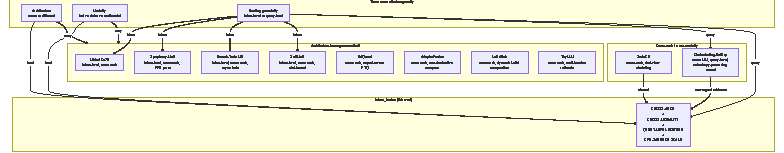
\includegraphics[width=0.95\textwidth]{figs/mermaid/heterogeneity_spectrum.pdf}
\caption{\textbf{异构谱系}——近期基础模型协作工作沿三轴展开：\emph{架构}（同 vs 不同）、\emph{模态}（文本 / 视觉 / 多模态）、\emph{路由粒度}（token-level vs query-level）。现有工作集中于架构同构的极限；架构异构的极限文献稀少，仅 ScaleKD 和 Orchestrating-HetExp 为最接近的前驱。本文工作在三条较难的轴的交叉处，且在 CPU 沙箱规模而非工业规模上。}
\label{fig:het-spectrum}
\end{figure}

\textbf{模型合并与稀疏化升级。}Task arithmetic \citep{ilharco2023}、TIES-merging \citep{yadav2023} 与 model soups \citep{wortsman2022} 合并的是共享主干的模型\emph{权重}。异构底座无法这样合并；我们的融合层就是异构情形下的对应机制，通过激活而非参数相加来工作。

\textbf{参数高效适配。}Adapter \citep{houlsby2019} 与 LoRA \citep{hu2022} 冻结底座、训练小型插入件。我们沿用同一哲学，但冻结的是一\emph{池}异构底座，训练的是底座之间的机器（投影、对齐器、路由器、中枢、门控）。AdapterFusion \citep{pfeiffer2021} 以非破坏方式组合逐任务 adapter，\citet{huang2024lorahub} 把这一思想推广到逐任务 LoRA 模块的动态线性组合——两者都示范了我们在跨架构融合中独立采用的非破坏性组合哲学。我们的对齐器阶梯可视为激活层面的对应物，而我们的多教师负面结果（\S\ref{sec:distill-exp}）呼应了 Pfeiffer 等的发现——朴素的多源组合并不免费。

\textbf{知识蒸馏。}蒸馏把教师行为迁移给更小的学生 \citep{hintonDistillingKnowledgeNeural2015,sanh2019,gou2021}；多教师变体亦已为人所知 \citep{you2017}，最新的多教师 LLM 蒸馏用推理链增强的目标函数恢复知识多样性 \citep{tian2025tinyllm}。嵌合蒸馏在两个方向上都不同：教师是一个多底座\emph{集成}——这一框架呼应 mixture-of-agents \citep{wang2024moa} 与堆叠泛化 \citep{wolpertStackedGeneralization1992}，但我们的协作发生在表示层、用可学习的路由与门控实现；学生只见一个底座的输入，却要复现集成的融合输出。量化感知训练在训练期注入伪量化噪声 \citep{dettmers2022}；我们把 INT4 伪量化用于专家输出，充当正则与硬件真实性压力，而非部署压缩声明。教师助手蒸馏 \citep{mirzadeh2020} 是我们在 \S\ref{sec:distill-exp} 分解的效应的最近类比：一个中间或更干净的目标会帮助学生，而这里的``更干净的目标''部分是直接目标项——我们证明它就是全部故事。

\textbf{选择机制的全局协调。}阶段二的问题——一个全局信号是否应当协调某种选择机制——由来已久。全局工作空间理论 \citep{baarsCognitiveTheoryConsciousness1988} 为广播式中枢提供了动机，但我们把它视为设计灵感而非可检验预测，因为它本身并未规定这种交互的函数形式。稀疏门控 MoE \citep{shazeerOutrageouslyLargeNeural2017} 与 Linformer 式全局混合 \citep{wangLinformerSelfAttentionLinear2020} 是最接近的架构亲属。线性注意力与状态空间家族的全局混合器 \citep{katharopoulos2020,gu2022s4,gu2023mamba} 处于一条正交的轴上：它们在单个模型内跨\emph{序列位置}混合，用状态携带内容；而我们的中枢在一个位置上跨许多冻结模型的\emph{专家}轴协调，调制的是路由的\emph{确定性}——一个重新缩放 logits、不添加内容的标量温度，它按构造保序，并在关闭时精确退化。携带内容的状态一般不满足这两条性质，因此两种机制是可组合的而非竞争的。

\section{方法一：异构子层融合}
\label{sec:method}

\subsection{问题设定}
\label{sec:setup}

设 $\mathcal{B} = \{B_1, \dots, B_M\}$ 为 $M$ 个冻结预训练底座，隐藏宽度为 $D_m$，一般具有不同架构：一个双向编码器（TinyBERT，$D{=}312$）\citep{jiao2020,devlin2019}、一个因果解码器（TinyLlama-110M，$D{=}768$）与一个视觉 Transformer（ViT-tiny，$D{=}192$）\citep{dosovitskiy2021}。每个底座使用自己的 tokenizer 或处理器并原生地产生隐藏状态 $h_m \in \R^{S \times D_m}$；我们从不强迫共享编码器。目标是一个工作在宽度 $D_{\text{shared}} = 256$ 的共享空间的融合层，使得 (i) 每个底座保持冻结，(ii) 只有对齐、路由与门控参数参与训练，(iii) 该层优雅降级——禁用任一单专家后系统仍能工作。

\subsection{异构融合层}
\label{sec:layer}

\begin{figure}[htbp]
\centering
\resizebox{\textwidth}{!}{%
\begin{tikzpicture}[
  font=\scriptsize, >=Stealth, node distance=3mm,
  base/.style={draw, rounded corners=1.5pt, align=center, inner sep=3.5pt, fill=blue!8, minimum width=34mm},
  stage/.style={draw, rounded corners=1.5pt, align=center, inner sep=3.5pt},
  aligner/.style={stage, fill=orange!16},
  router/.style={stage, fill=green!14},
  expert/.style={stage, fill=green!7},
  hub/.style={stage, fill=red!8},
  fuse/.style={stage, fill=orange!9},
  student/.style={stage, fill=violet!10},
  lbl/.style={font=\tiny, align=center},
]
\node[base] (bert) at (0, 1.45) {文本底座：TinyBERT\\ 双向编码器, $D_m{=}312$};
\node[base] (llama) at (0, 0) {代码底座：TinyLlama-110M\\ 因果解码器, $D_m{=}768$};
\node[base] (vit) at (0, -1.45) {图像底座：ViT-tiny\\ 视觉 Transformer, $D_m{=}192$};
\node[lbl, above=0.6mm of bert] {全部底座参数冻结};
\node[lbl, below=0.6mm of vit] {训练：对齐、中枢、路由、门控（以及学生的 LoRA）};

\node[aligner] (alg) at (4.35, 0) {跨架构对齐\\ 矩形 $P_m \in \R^{256 \times D_m}$\\ 或语义对齐器};

\node[hub] (hub) at (8.55, 1.95) {全局中枢 $c$\\ 门控式：$\tau = 1{+}\epsilon\tanh(W_t^\top c)$};
\node[router] (rout) at (8.55, 0.75) {稀疏路由器\\ $\hat\alpha = \topk(\softmax(x W_r^\top/\tau), K{=}1)$\\ 直通梯度};
\node[expert] (exp) at (8.55, -1.15) {冻结 SwiGLU 专家 $F_m$\\ + INT4 伪量化噪声\\ 逐专家 $\gamma_m, \beta_m, \alpha_m$};

\node[fuse] (fu) at (12.35, 0) {残差融合\\ $y = x + \sum_m \hat\alpha_m \alpha_m F_m^{\text{INT4}}$};

\node[student] (stu) at (12.35, -2.55) {独立学生\\ 单底座 $+$ LoRA（训练 $0.60\%$）};
\draw[->, densely dotted, thick] (fu.south) -- node[lbl, right=1.5pt, align=left] {嵌合\\ 蒸馏} (stu.north);

\draw[->] (bert.east) -- ($(alg.west)!0.5!(alg.north west)$);
\draw[->] (llama.east) -- (alg.west);
\draw[->] (vit.east) -- ($(alg.west)!0.5!(alg.south west)$);
\draw[->] (alg.east) -- (rout.west);
\draw[->] (alg.east) -- (exp.west);
\draw[->, densely dashed] (hub.south) -- node[lbl, left=1pt] {调制 $\tau$} (rout.north);
\draw[->, densely dashed] (rout.south) -- node[lbl, left=1pt] {选择} (exp.north);
\draw[->] (rout.east) -- (fu.140);
\draw[->] (exp.east) -- (fu.220);
\end{tikzpicture}}%
\caption{异构微观融合、协调式路由与嵌合蒸馏。三个架构与隐藏宽度各异的冻结预训练底座被原生编码、对齐进一个 256 维共享空间，并以稀疏（$K{=}1$）方式路由到冻结的 SwiGLU 专家，其输出携带 INT4 伪量化噪声。一个全局中枢调制共享路由器的 Softmax 温度（\S\ref{sec:hub}）。嵌合蒸馏随后把集成坍缩为一个独立的单底座学生（\S\ref{sec:distill}）。}
\label{fig:overview}
\end{figure}

图~\ref{fig:overview} 展示了该层。给定残差流输入 $x \in \R^{B \times S \times D_{\text{shared}}}$，每个专家 $m$ 计算
\begin{align}
\label{eq:expert}
h_m &= \stopgrad(x) \odot \gamma_m + \beta_m, \qquad
\tilde F_m = Q_{\text{INT4}}\big(F_m(h_m)\big), \\
F_m(h) &= \big(\mathrm{SiLU}(h W^{\text{gate}}_m) \odot (h W^{\text{up}}_m)\big)\, W^{\text{down}}_m,
\end{align}
其中 $Q_{\text{INT4}}$ 是分组（组大小 128）4 bit 伪量化，反向传播用直通估计器。三个刻意的设计选择塑造了该层。

\textbf{梯度截断。}专家输入被 detach（$\stopgrad$），因此冻结底座的中间激活从不进入计算图。激活显存从 $O(M L D_{\text{ff}})$ 降到 $O(L D_{\text{shared}})$ 加适配器参数——这正是 $M$ 底座融合能在 CPU 上训练的原因。代价是专家无法通过梯度塑造上游表示；适应全部由路由器与门控承担。

\textbf{带直通梯度的稀疏路由。}路由器从\emph{干净}的无噪声输入计算 logits $z = x W_r^\top$，$\alpha = \softmax(z/\tau)$，硬选择 $\hat\alpha = \topk(\alpha, K)$（除非另有说明，$K{=}1$）在前向施加，反向则沿 Softmax 权重回传，取直通估计器之意 \citep{bengio2013}。在干净输入上路由，可避免路由器决策去追逐它自己引入的量化噪声。温度 $\tau$ 是中枢唯一的施加通道，除拟合中枢外恒为 $1$（\S\ref{sec:hub}）。

\textbf{带正门控的残差融合。}层的输出为
\begin{equation}
\label{eq:fuse}
y = x + \sum_{m=1}^{M} \hat\alpha_m \, \alpha_m \, \tilde F_m(h_m),
\end{equation}
初始化时 $\alpha_m \sim \mathcal{U}(0.01, 0.1)$。正值、非平凡的门控初始化避免了近零门控死锁：以 $10^{-4}$ 量级初始化的门控收到过小梯度而无法逃逸——在采用均匀初始化之前，我们观察到过平直的训练曲线。

\subsection{两阶段训练协议}
\label{sec:training}

路由在训练早期很脆弱——随机路由器权重产生的噪声选择会毒化专家门控。因此训练分两阶段。\textbf{阶段 1}（前 $10\%$ 步）：路由被强制为均匀（$\hat\alpha_m = 1/M$，detach）且路由器冻结，只有对齐与门控参数学习。\textbf{阶段 2}（其余 $90\%$）：路由器解锁、Top-$K$ 选择激活，损失为
\begin{equation}
\label{eq:loss}
\mathcal{L} = \mathcal{L}_{\text{task}} + \lambda_1 \mathcal{L}_{\text{balance}} + \lambda_2 \mathcal{L}_{z},
\end{equation}
其中 $\mathcal{L}_{\text{balance}}$ 鼓励专家负载均衡，$\mathcal{L}_{z}$ 正则化路由器 logits。优化器分组隔离学习率：路由器与中枢 $10^{-4}$，对齐参数 $10^{-2}$，输出门控 $\alpha_m$ 为 $10^{-3}$。路由器必须慢，因为它的选择是离散的；对齐层可以快，因为它们的梯度是稠密的。

\subsection{对齐器阶梯}
\label{sec:align}

共享空间是异构底座相遇之处，而它的构造方式最终比栈中任何其他东西都更关键。我们评估四种复杂度递增的设计（图~\ref{fig:ladder-chain}）：

\begin{description}[leftmargin=1.4em, itemsep=1pt]
    \item[线性投影（基线）。]每个底座的隐藏状态经过一个矩形投影 $P_m \in \R^{D_{\text{shared}} \times D_m}$，正交初始化并冻结。各底座独立投影，互不知情。
    \item[均值对齐器。]逐底座的可学习降维 $W_m \in \R^{d \times D_m}$，随后对投影后的表示取跨底座均值。
    \item[跨架构注意力对齐器。]每个底座被投影到共享宽度；跨底座均值提供共享的键与值；每个底座用自己的查询投影向共享上下文发问——即跨注意力标准的 Q/K/V 分离 \citep{vaswani2017}——并残差式地加回被注意力聚合的概念向量。于是每个底座都读到一个由\emph{所有}底座共同书写的概念摘要。
    \item[Mixture 对齐器。]每个底座贡献 $n{=}4$ 个小型共享专家（两层 MLP），汇聚成一个 $M \times n$ 的专家池。专家输出作为查询，向由它们的均值导出的共享键/值上下文发问，聚合被注意力的输出。对齐器自身成为一个作用于异构来源之上、极小的 mixture-of-experts。
\end{description}

\begin{figure}[htbp]
\centering
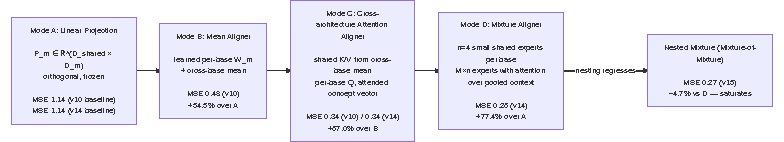
\includegraphics[width=0.95\textwidth]{figs/mermaid/alignment_ladder.pdf}
\caption{\textbf{对齐器阶梯}是一条严格但饱和的链：模式 A（线性投影）$\rightarrow$ B（均值对齐器）$\rightarrow$ C（跨架构注意力）$\rightarrow$ D（mixture-of-experts 对齐器）。每种模式在 5 种子 MSE 上都优于前一种；嵌套 mixture 退步 $4.7\%$（\S\ref{sec:align-exp}），标记天花板。}
\label{fig:ladder-chain}
\end{figure}

两个经验事实为阶梯提供动机。第一，\emph{原生编码不是可选项}：在一个早期对照中，三个模态全部由同一个 BERT 分词并编码，融合相对单专家的增益从 $+20.3\%$ 塌到 $+4.0\%$。统一编码恰好抹掉了路由器本该利用的架构差异。第二，阶梯是\emph{严格但饱和}的：每种模式优于前一种，而提升在 mixture 对齐器处停止（\S\ref{sec:align-exp}）——我们把这一天花板作为受规模限定的假设，而非定律。

\subsection{双通路路由：让 Attention 也可路由}
\label{sec:dualpath}

仅 FFN 的层在记忆库之间路由，却总是消费同一个 attention 输出。双通路扩展让 Attention 子层也可路由：每个 token 独立选择一个 \emph{attention 专家}与一个 \emph{FFN 专家}，两个池可以来自不同底座。Attention 专家暴露底座第一 block 的原生 Q/K/V/O 投影；被选专家的 attention 在其原生空间中重算，再经 $P_m$ 投影回来。逐专家优化器分组实现 \S\ref{sec:training} 的逐专家学习率隔离。双通路设计追问：跨架构互补性存在于 FFN 权重、注意力模式，还是两者？而 \S\ref{sec:fusion-exp} 的通路分解给出一个锋利的答案。

\section{方法二：协调共享路由器}
\label{sec:hub}

\subsection{四种中枢模式}
\label{sec:modes}

异构专家从未一起训练，对什么是好的路由决策意见不一。一个自然的应对是\emph{全局中枢}：一个概括整个集成、影响路由器的共享向量 $c \in \R^{D_{\text{shared}}}$。我们考虑中枢影响路由 logits $z_m$ 的四种方式：

\begin{definition}[广播模式]
$z_m^{(\text{bc})} = z_m + (U c)_m$，其中 $U \in \R^{M \times D_{\text{shared}}}$ 可学习。中枢给每个专家的 logit 加一个偏置。
\end{definition}

\begin{definition}[路由归一化模式]
$z_m^{(\text{rn})} = \mathrm{LayerNorm}(z_m + U c)$。先广播，再归一化。
\end{definition}

\begin{definition}[自适应 EMA 模式]
$\text{decay} = \sigmoid(\alpha \cdot \|c\|)$。中枢控制自己的指数移动平均衰减率；该 EMA 状态随后进入 logits。
\end{definition}

\begin{definition}[门控式模式（本文提出）]
$t_{\text{scalar}} = W_t^\top c$，$\tau = 1 + \epsilon \cdot \tanh(t_{\text{scalar}})$，$z_m^{(\text{g})} = z_m / \tau$。中枢调制 Softmax 温度。
\end{definition}

四种模式在\emph{如何}进入决策这一点上不同。广播与路由归一化向 logits \emph{加}入一个依赖中枢的项；自适应 EMA 让中枢塑造一个累积状态；只有门控式用一个正标量\emph{缩放} logits。这一结构性差异正是下一小节要转化为定理的东西。

\subsection{设计约束与为何只有门控式满足}
\label{sec:theory}

我们形式化五条任何面向冻结专家路由器的中枢机制都应满足的约束：
\begin{itemize}[leftmargin=1.5em, itemsep=1pt]
    \item \textbf{(G1) 完美退化}：$c=0$ 精确得到无中枢基线。
    \item \textbf{(G2) 保序}：中枢保持 logits 的相对顺序。
    \item \textbf{(G3) 单调性}：中枢强度单调地改变路由确定性。
    \item \textbf{(G4) 有界性}：中枢影响有理论上界。
    \item \textbf{(G5) 低开销}：中枢参数量为 $O(D_{\text{shared}})$，相对专家可忽略。
\end{itemize}

\begin{theorem}[完美退化]
\label{thm:deg}
当 $c=0$ 时，门控式精确等价于无中枢基线。
\end{theorem}

\begin{theorem}[保序]
\label{thm:order}
门控式保持 logits 的顺序；广播则可能将其颠倒。
\end{theorem}

\begin{theorem}[唯一性]
\label{thm:uniq}
在 \S\ref{sec:modes} 的四种中枢模式中，只有门控式同时满足全部五条约束 (G1)--(G5)。
\end{theorem}

证明梗概由结构直接得出，完整证明见附录~\ref{app:proofs}。定理~\ref{thm:deg} 成立是因为 $c=0$ 时 $\tau=1$；定理~\ref{thm:order} 成立是因为 $\tau \in (1-\epsilon, 1+\epsilon) \subset (0,\infty)$ 用同一个正标量去除所有 logits；定理~\ref{thm:uniq} 成立是因为广播违反 (G2)，路由归一化违反 (G1)（LayerNorm 即使在 $c=0$ 也会重新缩放），自适应 EMA 同时违反 (G1) 与 (G2)（其状态持续存在并携带内容）。

两条附注决定这些定理应如何被阅读。第一，它们是函数形式的\emph{构造性}性质而非经验主张，因此任何训练或数据泄漏都无法制造或摧毁它们；它们是本节中 \S\ref{sec:oos} 的样本外纪律无法触及的部分。第二，该定理关乎\emph{可容许性}而非哪种模式获胜：它的意思是，若一个中枢必须永不损害无中枢基线、且永不颠倒专家偏好，则四种模式中只有门控式可行。可容许的那个是否也恰好是表现最好的，是一个经验问题——而 \S\ref{sec:hub-exp} 表明答案并非简单的``是''。

\subsection{一个隐藏失效模式：tanh 饱和}
\label{sec:diagnosis}

跨项目工程世代的系统性实验揭示了一个中枢悄悄失效的情形。在长时程训练下，中枢停止更新：诊断运行显示 $\text{grad\_norm\_central} = 0.0000$，即 $c$ 与 $W_t$ 收到零梯度，冻结在一个次优值上。

根因是 \emph{tanh 饱和}。温度标量为 $\tau = 1 + \epsilon \cdot \tanh(t_{\text{scalar}})$，当 $|t_{\text{scalar}}|$ 变大时 $\tanh(t_{\text{scalar}}) \approx \pm 1$，其导数消失：
\begin{equation}
\frac{\partial \tau}{\partial t_{\text{scalar}}} = \epsilon \cdot (1 - \tanh^2(t_{\text{scalar}})) \approx 0 .
\end{equation}
由链式法则，$\partial \mathcal{L}/\partial c \approx 0$。前向照常运行，反向被切断。两种修复直接针对该机制：把 $\tanh$ 换成 $\softplus$（在同参数化下其导数在大的自变量处不消失），以及把梯度重新缩放注入中枢。两者都恢复了梯度流；\S\ref{sec:repair-exp} 报告它们对端到端误差做了什么、没做什么。

\section{方法三：重构独立模型}
\label{sec:distill}

子层层面的融合让每个底座都留在推理路径上。部署时我们要的恰好相反：一个模型、一个模态、没有集成。嵌合蒸馏把集成压缩为一个从不接触其他底座输入的单底座学生。

\textbf{学生架构。}单模态学生是真实的冻结 TinyBERT \citep{jiao2020}，在其隐藏状态上接一个秩 8 的 LoRA 适配器（$\alpha{=}16$），加一个到 $D_{\text{shared}}$ 的线性头与一个 LayerNorm。${\sim}14$M 参数中只有 $85{,}632$（$0.60\%$）可训练。与最初尝试的简化 MLP 学生不同，预训练学生为重建问题带来了先验语言学结构。

\textbf{蒸馏目标。}教师是带 mixture 对齐器的多底座融合系统。给定一批\emph{仅来自学生模态}的数据，教师跑完整的多底座前向，学生须与之匹配：
\begin{equation}
\label{eq:distill}
\mathcal{L}_{\text{distill}} = \alpha_{\text{h}} \, \mathrm{MSE}\big(y_s,\, \stopgrad(y_t)\big) + \beta_{\text{h}} \, \mathrm{MSE}\big(y_s,\, y_{\text{target}}\big),
\end{equation}
其中 $\alpha_{\text{h}} = 0.7$、$\beta_{\text{h}} = 0.3$。第一项蒸馏教师的隐藏状态概念方向；第二项加入直接目标信号。这不是温度缩放的 KL 散度，而是两个 MSE 项的加权组合，而权重 $\beta_{\text{h}}$ 正是 \S\ref{sec:distill-exp} 分解的对象。

\textbf{多模态学生。}多模态学生把 TinyBERT（文本）与 ViT-tiny（图像）配对，各配自己的 LoRA，再加一个决定哪一底座处理哪一输入的可学习模态路由器。它与单教师集成用同一目标训练。

\textbf{评估纪律。}我们最早的真实学生实验在训练分布输入上评估、目标容易拟合，产生了近零 MSE——一个伪装成成功的过拟合假象。此后所有学生评估都使用真实小语料的留出输入（16 句 Wikipedia 风格训练句，留出 6 句），迫使学生在它从未训练过的 token 分布下复现教师的概念方向。我们明确标出这一修正，因为未修正的数字漂亮到毫无意义，也因为同一条修正在栈中其他地方会朝两个方向改变结论（\S\ref{sec:oos}）。

\section{实验}
\label{sec:exp}

\subsection{实验设置与诚实的边界}
\label{sec:exp-setup}

全部实验在 CPU-only（Linux，PyTorch 2.x，无 GPU 加速）上完成。宽度很小（$D_{\text{shared}}{=}256$，$S{=}16$），目标是合成的类方向构造（共享空间的一块被置为 $1.0$ 表示目标类），除另有说明每个配置取 5 个种子。全栈通过 430 个单元与集成测试；下文每个数字都由一个具名、已提交的脚本产生（复现命令见 \S\ref{sec:repro}）。这些是\emph{机制层面}的结果：它们确立的是重构机制在受控条件下按设计工作，而非该方法能经受 0.5B 参数规模或真实任务上的困惑度级评估。我们把规模差距视为最大的开放风险，并在 \S\ref{sec:limitations} 讨论。

\subsection{子层融合增益及其来源}
\label{sec:fusion-exp}

\begin{table}[htbp]
\centering
\caption{异构底座的子层融合（5 种子均值，fuse MSE；越低越好）。v6：三架构上的仅 FFN 路由。v7-A/v7-B：双通路路由（每 token 一个 attention + 一个 FFN 专家），分别为跨架构与同架构。增益按种子计算后平均。}
\label{tab:fusion}
\small
\setlength{\tabcolsep}{4.5pt}
\begin{tabular}{lccccc}
\toprule
\textbf{设置} & \textbf{仅 attn} & \textbf{仅 ffn} & \textbf{平均} & \textbf{fuse} & \textbf{相对平均增益} \\
\midrule
v6：仅 FFN，跨架构（3 底座） & --- & 7.08 & 6.77 & \textbf{5.60} & $+17.3\%$ \\
\quad 相对最佳单专家增益 & & & & & $+20.3\%$ \\
v7-A：双通路，跨架构 & 1.16 & 7.10 & 7.06 & \textbf{1.06} & $+84.8\%$ \\
v7-B：双通路，同架构 & 0.382 & 0.414 & 0.383 & \textbf{0.378} & $+1.0\%$ \\
\bottomrule
\end{tabular}
\end{table}

表~\ref{tab:fusion} 汇总融合结果。仅 FFN 路由（v6）下，融合层超出最佳单专家 $20.3\%$、超出等权平均 $17.3\%$，每个种子都通过——这是首次证明真正不同的预训练架构可以在子层层面共享同一个稀疏路由器。双通路路由（v7-A）把相对平均的裕度提升到 $84.8\%$。

通路分解是更有意思的部分，也是能在留出评估下存活的发现之一。在跨架构设定下，仅 attention 通路达到 MSE $1.16$——已接近融合的 $1.06$——而仅 FFN 通路（$7.10$）与平均（$7.06$）难以区分。跨架构互补性因此几乎全部显现在 \emph{注意力模式}里：一旦每个 token 能向架构与自己 attention 模式相配的那一个底座求教，FFN 专家的剩余贡献就只是残差精修。对这项主张的独立留出审计（\texttt{run\_v46\_attn\_path\_audit}）在 in-sample 与 held-out 两种协议下重测 attention 对 FFN 的通路差：in-sample 为 $+82.7\%$、held-out 为 $+70.6\%$，两种协议均 $5/5$ 全胜，故该主张并非 in-sample 评估的假象。我们狭义地陈述它——attention 跨架构的差异比 FFN 激活更大——且它与 FFN 的键值记忆观并不矛盾 \citep{geva2021,meng2022,dai2022}：FFN 权重\emph{在一个架构内}承载丰富知识，但我们的结果表明这些知识\emph{跨}架构时平均得很好，而注意力模式不行。在同架构对照（v7-B）中，三个 TinyBERT 仅由随机 Q/K/V/O 扰动区分，双通路增益缩小到 $+1.0\%$：架构多样性被移除后，路由器几乎没有可选择的余地。路由的价值来自架构多样性，而非专家数量。

\subsection{对齐器阶梯及其天花板}
\label{sec:align-exp}

\begin{table}[htbp]
\centering
\caption{对齐器阶梯（5 种子均值，fuse MSE）。每个区块是一次受控比较；mixture 对齐器使阶梯饱和，嵌套它没有帮助。}
\label{tab:ladder}
\begin{tabular}{llcc}
\toprule
\textbf{比较} & \textbf{对齐器} & \textbf{fuse MSE} & \textbf{相对下一档} \\
\midrule
\multirow{3}{*}{投影 vs.\ 语义（v10）}
 & 线性投影 & 1.0436 & --- \\
 & 均值对齐器 & 0.4753 & $+54.5\%$ \\
 & 跨架构注意力 & \textbf{0.3448} & $+67.0\%$ \\
\midrule
\multirow{3}{*}{注意力 vs.\ mixture（v14）}
 & 线性投影 & 1.1409 & --- \\
 & 跨架构注意力 & 0.3376 & $+70.4\%$ \\
 & mixture 对齐器 & \textbf{0.2575} & $+77.4\%$ \\
\midrule
\multirow{3}{*}{mixture vs.\ 嵌套（v15）}
 & 跨架构注意力 & 0.3216 & --- \\
 & mixture 对齐器 & \textbf{0.2525} & $+21.5\%$ \\
 & 嵌套（mixture of mixture） & 0.2645 & $-4.7\%$ \\
\bottomrule
\end{tabular}
\end{table}

\begin{figure}[htbp]
\centering
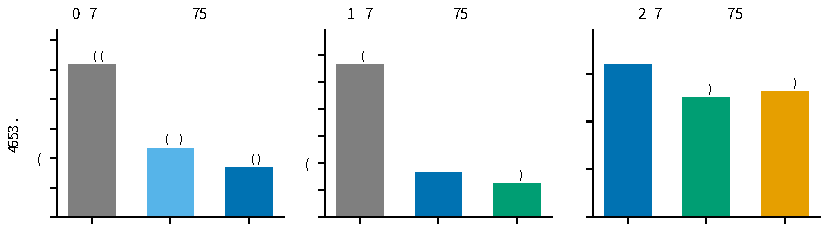
\includegraphics[width=\textwidth]{figs_zh/fig_alignment.pdf}
\caption{对齐器阶梯。(a) 语义对齐优于冻结线性投影；跨底座注意力优于均值。(b) mixture 对齐器优于单概念注意力。(c) 嵌套 mixture 对齐器略微退步：阶梯在一级跨专家注意力处饱和。越低越好。}
\label{fig:ladder-results}
\end{figure}

表~\ref{tab:ladder} 与图~\ref{fig:ladder-results} 展示了阶梯；图只是可视化表中的 5 种子均值，不引入新量。顺序 线性 $<$ 均值 $<$ 注意力 $<$ mixture 在每次比较中都严格成立，从线性基线到 mixture 对齐器的总爬升为 $-77.4\%$ MSE。负面结果与正面同样清晰：一个两级嵌套 mixture（mixture of mixture）落在注意力和 mixture \emph{之间}，比单级 mixture 对齐器差 $4.7\%$。跨底座注意力值一个层级；第二级层级增加参数、稀释共享概念上下文，却不增加表示能力。

一次组合测试把这一点钉得更实。我们把修复后的门控式路由器与注意力对齐器组合：相对它们共同的线性投影基线 $1.1625$，组合达到 $+71.0\%$ 增益（$0.3374$），而对齐器自己的配置达到 $+72.6\%$（$0.3191$）——相差不足 2 个百分点，但在全部 5 个种子上一致偏向对齐器一侧，处于种子波动之内。一旦对齐器已经提供了跨底座概念交换，路由器层面的修复就无事可做。栈中相邻层的改进不是可加的；第一个充分机制会吸收全部增益。

容量混杂已排除。四种对齐器的参数量不同（仅计对齐器参数：线性 $325{,}632$；注意力 $720{,}640$；mixture $2{,}291{,}968$；嵌套 $1{,}704{,}448$），因此我们做了一个容量匹配对照：把 mixture 对齐器缩减为每底座一个共享专家，得到恰好 $720{,}640$ 个参数——与注意力对齐器逐位相等。在匹配容量下，mixture 对齐器在留出数据上仍以 $+36.5\%$ 领先注意力对齐器（5 种子中位数；均值 $+28.8\%$；去掉最佳种子 $+33.5\%$；5/5 配对种子全胜），而把 mixture 的专家数从 $1$ 扫到 $8$——$6.09\times$ 的容量范围——留出 MSE 仅移动 $-5.6\%$ 且非单调。因此阶梯读作设计，而非规模。嵌套对齐器同样是一个表达力天花板而非容量天花板：在 $2.37\times$ 单专家 mixture 参数下，它差 $28.6\%$。仍然开放的是规模：整条阶梯测于 $D_{\text{shared}}{=}256$、三个底座与合成目标，因此饱和点是一个受规模限定的假设，在 $D_{\text{shared}}{\geq}768$、真实目标下确认或打破它，是优先级最高的后续实验。

\subsection{路由协调：in-sample 不等于样本外}
\label{sec:hub-exp}

表~\ref{tab:hub} 报告跨架构融合任务上的四种中枢模式，它是本文中最清楚的一个``in-sample 评估会得出错误结论''的案例。

\begin{table}[htbp]
\centering
\caption{跨架构融合上的中枢模式（\texttt{run\_v44\_hub\_modes\_audit}，5 种子配对中位数）。in-sample 与 held-out 两种排名在同一协议下读取。路由归一化同时领先两者；项目自己的主表曾记录为 in-sample 最优的模式（自适应 EMA）泛化落差最大、样本外垫底。}
\label{tab:hub}
\small
\setlength{\tabcolsep}{5pt}
\begin{tabular}{lcccc}
\toprule
\textbf{中枢模式} & \textbf{in-sample MSE} & \textbf{held-out MSE} & \textbf{held-out 增益} & \textbf{胜} \\
\midrule
广播（基线） & 0.3236 & 0.3538 & --- & --- \\
路由归一化 & \textbf{0.2835} & \textbf{0.3342} & $+4.3\%$ & $5/5$ \\
门控式 & 0.2983 & 0.3462 & $+5.8\%$ & $3/5$ \\
自适应 EMA & 0.2859 & 0.3573 & $+0.3\%$ & $3/5$ \\
\bottomrule
\end{tabular}
\end{table}

\begin{itemize}[leftmargin=1.4em, itemsep=2pt]
    \item \textbf{in-sample 表关于自己的冠军就已出错。}项目自己的主表把自适应 EMA 记为 in-sample 最优；审计（\texttt{run\_v44\_hub\_modes\_audit}，其绝对水平与早先那次运行略有差异）表明 in-sample 最小值其实是路由归一化（$0.2835$），而路由归一化也是 held-out 冠军（$0.3342$，相对广播 $5/5$ 配对全胜）。自适应 EMA——那个被记录的 in-sample 冠军——样本外塌到相对广播 $+0.3\%$、在 $2/5$ 种子上落败，且泛化落差在四者中最大（$+25.0\%$）。一次在不同规模的真实语料上的独立重跑（\texttt{run\_v25\_corpus\_central}）复现了该排序：路由归一化 held-out 最优（相对广播 $+4.6\%$），自适应 EMA 次之（$+2.0\%$），门控式为负（$-5.1\%$）。
    \item \textbf{门控式的可容许性并不使它成为经验冠军。}门控式中枢把中枢协调增益从 $-71.9\%$（广播）翻正到 in-sample $+44.5\%$，是四者中最大的 in-sample 改进。但在与上文相同的 held-out 协议下，该增益塌到 $+4.0\%$（3/5）。因此 \S\ref{sec:theory} 的定理与经验排名回答的是不同问题：门控式是唯一\emph{可容许}的模式，却不是样本外\emph{最优}的模式。
    \item \textbf{这里的容量混杂方向相反。}一个自然的担心是门控式取胜因为它参数更多。它反而更少：门控中枢携带 512 个参数，广播是 1{,}024，因此可容许性结果不可能被解释为容量效应。更何况完美退化与保序是构造性性质，无论如何都不可能由额外参数产生。
\end{itemize}

这一教训不止于这张表。四种中枢模式在 in-sample 上的差距与其种子波动相当，因此在这一尺度下的 in-sample 组合机制比较，衡量的是各机制\emph{拟合}得多好，而非它们能\emph{做}什么。held-out 协议才是区分二者的东西。

\subsection{语料规模边界未在样本外确立}
\label{sec:corpus}

本项工作早先曾宣称一条干净的语料规模边界：自适应 EMA 在极小与小型语料上取胜，门控式在中等与大型语料上取胜，交叉点在 16--32 训练样本（表~\ref{tab:scale}）。该边界在 in-sample 存在，但它没能经受同一场 held-out 检验。

\begin{table}[htbp]
\centering
\caption{语料规模扫描（v29），in-sample。\emph{下表这个表观边界并未在样本外确立}（\S\ref{sec:corpus}）；此处报告它，作为审计所更正的那条 in-sample 观察。}
\label{tab:scale}
\small
\begin{tabular}{lccc}
\toprule
\textbf{语料规模（训练/验证/测试）} & \textbf{in-sample 最优} & \textbf{MSE} & \textbf{held-out 最优} \\
\midrule
极小（8/4/4） & 自适应 EMA & 0.7035 & 自适应 EMA \\
小（18/6/6） & 自适应 EMA & 0.6984 & 自适应 EMA \\
中（32/12/12） & 门控式 & 0.6971 & \emph{未重跑} \\
大（64/24/24） & 门控式 & 0.7029 & 自适应 EMA \\
\bottomrule
\end{tabular}
\end{table}

只扫两个端点规模（\texttt{run\_v45\_scale\_boundary\_audit}；5 种子；训练与留出），边界在 in-sample 存在（自适应 EMA $\rightarrow$ 门控式），但 held-out 中位数在\emph{两个}规模上都给出自适应 EMA，即没有边界。更糟的是，在大规模档，两种读数彼此矛盾：非配对中位数把自适应 EMA 排第一，而配对逐种子比较把门控式排第一（自适应 EMA 只赢 $1/5$），矛盾由一个种子驱动——该种子上自适应 EMA 达到 $0.767$，而门控式是 $0.543$。因此我们报告该边界\emph{未在样本外确立}，而非已确认：四个规模档中有两个未重跑（包括交叉档本身），且小规模档的 held-out 裕度为 $3/5$ 种子上的 $+0.5\%$，即在噪声之内。确立或推翻该边界需要中间档与配对协议；现有数据不足以定论。

\subsection{tanh 饱和修复：梯度恢复，误差不变}
\label{sec:repair-exp}

\S\ref{sec:diagnosis} 的两种修复针对一个真实缺陷——长训练下 $\text{grad\_norm\_central} = 0.0000$——且两者都恢复了注入中枢的非零梯度。然而它们对端到端误差的影响在噪声之内，而只有 held-out 审计才让这一点可见。在审计协议下，softplus 修复使融合 MSE 变化 $-0.44\%$，梯度缩放修复变化 $-0.11\%$，两者均 $0/5$ 种子获胜：修复解决了\emph{机制}，却没有改变\emph{结果}。这是一个小而干净的、本文整体模式的实例——一个在诊断层面正确的修复，在指标层面仍可能不可见——也正是我们分开报告``修复''与``效果''、而不合并为一项主张的原因。

\subsection{嵌合蒸馏：裕度、泄漏分解与多教师}
\label{sec:distill-exp}

\begin{table}[htbp]
\centering
\caption{嵌合蒸馏（5 种子均值）。教师是带 mixture 对齐器的多底座融合集成。$\dagger$：在训练分布输入上评估；近零值是过拟合假象而非泛化。v18 在留出的真实 Wikipedia 文本上评估。}
\label{tab:distill}
\small
\setlength{\tabcolsep}{4.5pt}
\begin{tabular}{llccc}
\toprule
\textbf{学生} & \textbf{评估} & \textbf{教师} & \textbf{蒸馏后} & \textbf{相对教师} \\
\midrule
v13：MLP 学生（无预训练） & 训练分布目标 & 0.3245 & 0.3076 & $+5.4\%$ \\
v16：TinyBERT + LoRA（$0.60\%$） & 训练分布目标$^\dagger$ & 0.2764 & 0.1380 & $+50.1\%$ \\
v18：TinyBERT + LoRA & 留出真实文本 & --- & 0.1574 & 可行 \\
v21：BERT+ViT 多模态 & 训练分布目标$^\dagger$ & 0.3238 & 0.1620 & $+50.0\%$ \\
\bottomrule
\end{tabular}
\end{table}

\begin{figure}[htbp]
\centering
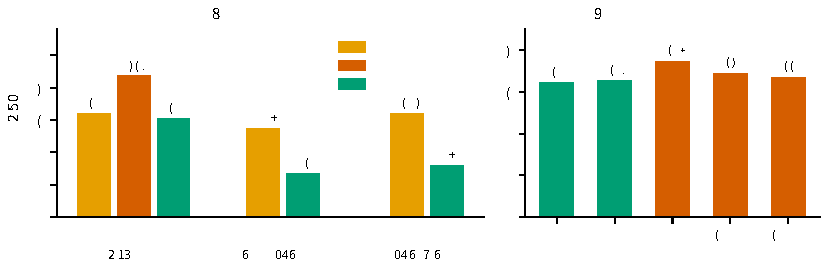
\includegraphics[width=\textwidth]{figs_zh/fig_distill.pdf}
\caption{(a) 单教师嵌合蒸馏：蒸馏学生在每种设置下都超出其多底座教师。(b) 多教师蒸馏在所有配置上退步（v17）；分派式改写消除了伤害但不产生增益（v40）。越低越好。}
\label{fig:distill}
\end{figure}

表~\ref{tab:distill} 报告蒸馏结果。模式一致，初看反直觉：蒸馏学生\emph{看起来}在复现融合输出上比教师产生它更擅长——MLP 学生 $+5.4\%$，TinyBERT 学生 $+50.1\%$（$0.138$ vs.\ $0.276$），多模态学生 $+50.0\%$（$0.162$ vs.\ $0.324$）。我们不按面值接受这一点，下文的分解表明也不应接受。

\textbf{复制为何会胜过原件，以及为何它没有。}教师的前向是随机的——硬 Top-$K$ 路由加每一步的 INT4 量化噪声——而学生被训练去匹配教师的\emph{期望}输出。一个拟合条件均值的函数，其 MSE 会低于它所模仿的含噪过程（Jensen 型间隙），因此一个确定性学生\emph{原则上应当}按构造胜过其随机教师。这给出三种候选解释——Jensen 型方差平均优势、$\beta_{\text{h}}=0.3$ 直接目标项、真正的概念方向传递——而每一种都可检验。

\textbf{检验一 —— $\beta_{\text{h}}$ 扫描。}令 $\beta_{\text{h}}=0$、其余不变，隔离出纯蒸馏（\texttt{run\_v32}）。在与本表相同的教师与评估协议下，纯蒸馏的 MSE 为 $0.324 \pm 0.013$，混合目标为 $0.165 \pm 0.007$，教师为 $0.323 \pm 0.015$。纯蒸馏\emph{并不优于教师}：逐种子配对间隙为 $-0.0009 \pm 0.0038$（10 个种子的均值 $\pm$ 标准差；不显著）。把 $\beta_{\text{h}} \in [0,1]$ 以 $0.1$ 步长扫描，学生 MSE 从 $0.317 \pm 0.040$ 单调降到 $0.000 \pm 0.000$，在 $\beta_{\text{h}}=0.3$ 处无跳变，故该项的效果与其权重成正比——一个饱和的插值，而非某种可在临界点之上被恢复的阈值机制。在多模态学生上做同样的扫描（\texttt{run\_v42}）复现了这一模式，从 $\beta_{\text{h}}{=}0$ 的 $0.3270$ 到 $\beta_{\text{h}}{=}1$ 的 $0.0001$；在 $\beta_{\text{h}}{=}0$ 处多模态学生为 $0.3270$，教师为 $0.3255$，即 $-0.5\%$，$5/5$ 种子未能胜过教师。

\textbf{检验二 —— 方差平均是有界的。}把教师换成一个在 20 次不同随机输入上前向取平均的\emph{超确定性}版本（\texttt{run\_v32.3}），其 MSE 不变（$0.324 \pm 0.015$，与确定性教师完全相同），纯学生相对它的间隙为 $-0.0008 \pm 0.0038$——同样不显著。在这一尺度上平均 20 次前向并不改变教师输出，故 Jensen 型机制在此没有可测量的贡献。

\textbf{检验三 —— 表示迁移未发现混合优势。}若混合目标已教给学生教师内部的概念方向，这些方向应当迁移。在同一教师下训练混合与纯学生后，我们冻结两个学生的 LoRA 参数，把输出头换成新的随机线性分类器，在一个新生成的目标集上训练该头，并比较准确率（\texttt{run\_v32.4}）：混合学生达到 $0.733 \pm 0.065$，纯学生达到 $0.767 \pm 0.102$——纯学生反而略好，差异不显著。

三项检验一致。$50\%$ 上下的表观裕度没有一分归因于概念方向传递或方差平均；混合目标下的全部实测优势都归因于 $\beta_{\text{h}}=0.3$ 的直接目标项。真正携带机制证据的对比是\emph{学生之间}在同一个随机教师下的对比：MLP 学生只闭合了 $+5.4\%$ 的间隙，TinyBERT 学生 $+50.1\%$，多模态学生 $+50.0\%$。该排序反映的是预训练先验与泄漏目标信号之间的交互，而非教师概念方向的内化。由于 v32 重跑使用与原始 v16 记录略有不同的绝对水平（教师 $0.324$ vs.\ $0.257$；混合学生 $0.164$ vs.\ $0.138$），我们在内部自洽的 v32 运行内解读该分解，不把其水平与表~\ref{tab:distill} 交叉比较；我们保留 v16 协议行以保证正面结果的可复现。

v18 的留出修正指向同一方向。在留出真实 Wikipedia 文本下，蒸馏学生保持 MSE $0.157$，而假词表与仅微调两个对照都停在 $\approx 0$——并非因为它们泛化，而是因为它们的评估输入与目标平凡可拟合。学生的 $0.157$ 正反映了在混合目标下对教师输出的拟合；上文泄漏分解表明这就是它的全部。

\textbf{多教师蒸馏失败，改写它也无济于事。}一个自然的下一步是同时从若干教师（注意力对齐器教师、mixture 教师、嵌套教师）蒸馏，或许带权重。每个配置都退步（图~\ref{fig:distill}(b)）：两个教师 $-15.8\%$，三个教师 $-6.3\%$，加权三教师 $-3.9\%$（相对单教师）。教师们在所传递概念空间的\emph{方向}上存在分歧；容量受限的学生无法对齐冲突的目标，而平均信号又稀释了每个教师的专门化。一个把加权和换成逐样本分派的分派式改写（\texttt{run\_v40\_dispatch}）检验了如下假设——失败是回归\emph{形式}的假象，而非多教师蒸馏本身。它是部分修复：分派消除了加权组合的\emph{伤害}（中位数 $0.3344 \rightarrow 0.3195$），但没有产生相对单教师的增益，且三种形式——加权、均值、轮转分派——彼此难以区分（中位数 $0.3335$--$0.3398$）。教师侧合计约保有 $13\%$ 的互补余量，而\emph{我们尝试的任何形式都无法把它传给学生}。一个分派 oracle 臂显示均值增益 $+6.0\%$，但中位数塌到 $+0.6\%$、去掉最佳种子 $+1.1\%$——一个我们不予引用的单种子假象。结论比``多教师蒸馏不好''更窄：当教师共享同一数据与目标、没有领域划分时，它们表面的分歧是噪声，失败是学生侧的容量天花板，而非可修的聚合假象。

\subsection{任务级评估：一条边界，而非一个结果}
\label{sec:vqa-exp}

我们尝试用一个小型 VQA 基准从概念重建走向真实任务。4 个简单类别下，仅图像学生靠一个模态捷径达到 $100\%$ 准确率，多模态学生达到 $91.7\%$：任务无法区分多模态推理与单模态作弊。我们随后用 8 个旨在击败捷径的陷阱类别重建基准。所有模型——仅文本、仅图像、多模态——都恰好跌到 $50\%$，即随机猜测的准确率。把任务难度加倍没有暴露出多模态能力。我们报告两种读法。有利的读法：24 个训练样本、CPU 规模的学生，基准无法训练出跨模态接地，因此随机水平的准确率衡量的是基准而非融合层。不利的读法，我们无法排除：一个多模态学生在被设计为需要跨模态推理的任务上未能超过随机，可能是该机制自身的能力边界。分辨这两种读法，正是我们基于 CLIP \citep{radford2021} 的教师流水线——已备好但尚未完成端到端运行——的目的。

\subsection{样本外纪律：什么存活，什么不存活}
\label{sec:oos}

上文各项审计并非一堆杂散的更正；合起来，它们是关于这类组合机制应如何评估的单一方法论结果。我们实施了一套统一的样本外协议（\texttt{run\_v44}--\texttt{run\_v47}；对每一仍标记为 pending 的主张，都用同分布的留出划分、外加一次不同规模的真实语料重跑），并按是否存活的把栈中的发现分类。

\begin{table}[htbp]
\centering
\caption{按 held-out 协议下的存活情况排序的发现。``保留率''是样本外剩余效应占 in-sample 效应的比例。}
\label{tab:oos}
\small
\setlength{\tabcolsep}{4.5pt}
\begin{tabular}{p{0.40\textwidth}ccc}
\toprule
\textbf{发现} & \textbf{in-sample} & \textbf{held-out} & \textbf{判定} \\
\midrule
attention 通路优势（v46） & $+82.7\%$ & $+70.6\%$ & \textbf{存活} \\
对齐器阶梯天花板（v41） & 相对 attn $+36.5\%$ & 容量匹配 & \textbf{存活} \\
中枢：路由归一化最优（v44） & 最优 & 最优（$5/5$） & \textbf{存活（已更正）} \\
中枢：门控式协调增益（v43） & $+44.5\%$ & $+4.0\%$ & 收缩到噪声 \\
语料规模边界（v45） & 存在 & 不存在 & \textbf{未确立} \\
长训练增益（v19） & $+4.3\%$ & $+1.5\%$ & 收缩（保留 $34\%$） \\
梯度修复（v30/v31） & $-0.44\%$ / $-0.11\%$ & 相同 & 无效果 \\
\bottomrule
\end{tabular}
\end{table}

表~\ref{tab:oos} 是本文最可迁移的结果，且不专属于我们的架构。存活下来的是有\emph{机制}理由存活的东西：attention 通路优势反映了 Transformer 的一条结构性质（注意力模式跨架构的差异大于 FFN 激活），对齐器阶梯天花板则是一条匹配容量的设计陈述。失败的是拟合优势：中枢模式排名、语料规模交叉、以及来自长训练或来自``对一个端到端效应在噪声之内的机制所做的修复''的增益。我们把它作为一条给同行的经验法则提出：在冻结底座组合的小规模场景下，报告 held-out 排名而非 in-sample 排名，并把任何与种子波动相当的裕度视为未决。

\section{讨论}
\label{sec:discussion}

\textbf{四条设计原则。}这些结果背后的系统性迭代稳定为四条原则。我们把它们陈述为从一个系统提炼出的领域性启发法——推广到其他架构是假设而非结论——但我们预期它们比具体配置走得更远。(1)~\emph{让异构性可分可合}：每个组件（路由器、门控、对齐器、中枢、每条通路）都能独立启停，这正是本文每次消融都只是一行开关的原因。(2)~\emph{负面结果是地图边界}：组合、嵌套、多教师与 VQA 的失败，比任何正面结果都更锋利地界定了该方法。(3)~\emph{冻结底座组合要求机制层面的诊断}：因为底座不更新，消融必须直达子层机制——路由器、门控、对齐器、中枢、伪量化——而组件级的命名正是我们把这些诊断彼此分开的方式；我们刻意避免用不同的认知或生物类比去命名同一个机制。(4)~\emph{增量扩展}：每一代都复用上一代冻结的组件，这正是在架构成长的过程中让 430 个测试保持通过的原因。

\textbf{反复出现的规律：更多不等于更好。}在五项独立比较中，增加机制——更多的路由器修复、第二级对齐器、更多教师、更难的 toy 任务——要么毫无作用、要么有害。有效的机制（原生编码、共享 K/V 注意力、一级 mixture、单一教师）每一个都\emph{替换}了更弱的东西，而不是叠加其上。对子层层面的重构，浮现出的实用配方是：原生编码，用一级 mixture 对齐，稀疏路由，只用可容许的中枢协调路由器，从单一教师蒸馏——然后停手。

\textbf{样本外纪律作为统一方法。}本文三个阶段与其说由架构统一，不如说由评估统一。每个阶段都提出一个容易在 in-sample 为真、却难以在样本外为真的主张，而 \S\ref{sec:oos} 的审计表明，栈中约有一半的 in-sample 发现未能存活。我们依赖的两条性质对此免疫，因为它们是构造性的而非经验的——完美退化与保序是一个函数形式的性质——因此我们全程把这类性质与测量得到的性质分开。这种分离，而非任何一个数字，才是我们要带到下一个系统中的东西。

\textbf{关于数据规模与融合策略的跨论文信号。}四条独立的近期工作报告了一个相关模式：小数据与小模型偏好\emph{注入式}组合（完整路由器、分离适配器、粗粒度路由），而大数据与大模型偏好\emph{平均式}组合（加权组合、全微调、加性合并）。AdapterFusion \citep{pfeiffer2021} 在训练数据稀缺时凸显这一取舍；Mixtral 式稀疏路由 \citep{jiang2024mixtral} 恰在死专家塌缩变得灾难性的地方要求负载均衡；\citet{liu2026orchestrating} 的粗粒度路由出于我们这里不存在的延迟原因收敛到整查询决策，却导向同一架构选择；Branch-Train-MiX \citep{sukhbaatar2024btx} 在有限算力下由其 MoE 微调阶段主导。我们的四模式比较在单一训练规模下完成，与该假设一致，但我们自己的留出审计（\S\ref{sec:corpus}）表明，该边界的\emph{文内}版本并未确立——这本身就是我们把数据规模依赖性陈述为文献汇聚假设而非发现、并把跨训练规模的文内扫描留给未来工作的原因。

\textbf{与路由协调问题的关系。}共享路由器应如何协调——用哪种中枢模式，以及该选择如何与数据规模交互——是 \S\ref{sec:hub} 的主题。我们的答案干净地分为两部分：已证明的可容许部分（门控式是唯一满足 G1--G5 的模式）与仍然开放的经验部分（在我们的尺度下样本外最优的是路由归一化，而该排序能否持续到工业规模未经检验）。

\section{局限性}
\label{sec:limitations}

规模是首要局限。全部结果为 CPU 沙箱结果：$D_{\text{shared}}{=}256$、序列长度 16、合成类方向目标而非语言模型困惑度、toy 规模语料；本文没有任何结论确立 0.5B+ 参数或真实下游基准上的行为。INT4 伪量化是训练期的噪声注入，不是部署核。Attention 专家只读取底座的第一 block，没有层选择研究。Top-$K$ 固定为 $K{=}1$。语料规模边界是\emph{未决}而非被推翻：四个规模档中有两个以及交叉档本身未在样本外重跑。任务级多模态评估仍然开放。最后，蒸馏裕度是在教师自身目标分布上的重建 MSE 中测量的；分解表明它们就是目标泄漏，而任何真正的传递能否转化为下游能力未经检验。

\section{结论}
\label{sec:conclusion}

我们分三个阶段重构了冻结的异构预训练模型：一个子层融合层，通过共享稀疏路由与语义对齐器在冻结架构专家之间路由 token；一套协调理论，指出温度调制是唯一既能精确退化、又能保序、有界、且参数量为 $O(D_{\text{shared}})$ 的中枢机制；以及嵌合蒸馏，把集成坍缩为一个独立学生。对齐空间有一条严格阶梯，其天花板在一级 mixture 处，容量匹配对照表明它来自设计而非规模；跨架构融合增益集中于 attention 通路，该主张在留出评估下存活。嵌合蒸馏表观的``学生优于教师''裕度全部归因于损失中的直接目标项，而非概念方向传递或方差平均。负面结果——无可加组合、无嵌套增益、无多教师增益、可容许中枢在样本外无优势、toy 基准停在随机——与正面结果同样锋利地限定了该方法。我们最后的贡献是方法论上的：一套统一施加于全栈的样本外纪律，推翻了我们自己的若干 in-sample 发现，同时让机制性的那些完好无损。开放的前沿是规模：这些机制现已在 CPU 尺度上被明确、被检验、被界定，它们在预训练尺度上的行为是下一个要紧的问题。

\section*{可复现声明}
\label{sec:repro}

全部实验均以脚本形式置于项目仓库中。核心复现命令：

\begin{itemize}[leftmargin=1.6em, itemsep=0.5pt, parsep=0pt]
    \item 融合与通路分解：\texttt{bash run.sh v6}、\texttt{run.sh v7a}、\texttt{run.sh v7b}；attention 通路审计 \texttt{run\_v46\_attn\_path\_audit.py}。
    \item 对齐器阶梯：\texttt{examples/run\_v10\_aligner.py}、\texttt{run\_v14\_aligner\_compare.py}、\texttt{run\_v15\_mom\_compare.py}；容量对照 \texttt{run\_v41\_capacity\_audit.py}。
    \item 路由协调：\texttt{run\_v22\_theory\_compare.py}、\texttt{run\_v43\_central\_audit.py}、\texttt{run\_v44\_hub\_modes\_audit.py}、\texttt{run\_v45\_scale\_boundary\_audit.py}。
    \item 蒸馏：\texttt{run\_v13\_distill.py}、\texttt{run\_v16\_bert\_distill.py}、\texttt{run\_v18\_wiki\_distill.py}、\texttt{run\_v21\_multimodal\_distill.py}、\texttt{run\_v32\_leakage\_audit.py}、\texttt{run\_v40\_dispatch.py}。
    \item 留出审计：\texttt{run\_v47\_central\_heldout.py}、\texttt{run\_v47\_scale\_hetero\_heldout.py}。
    \item VQA 边界：\texttt{examples/run\_v23\_vqa\_distill.py}、\texttt{run\_v23\_vqa\_hard.py}。
\end{itemize}

完整测试套件（\texttt{bash run.sh test}）运行 430 个单元与集成检查。环境：Linux、Python 3.11、PyTorch 2.x、CPU-only，每个配置 5 个种子。

\section*{AI 辅助披露}

稿件撰写由一个 AI 写作代理在项目的实验记录与规范之上辅助完成；全部实验结果、代码与设计决策均为作者本人所作。

\bibliographystyle{plainnat}
\bibliography{reconstruct}

\appendix

\clearpage

\section{超参数}
\label{app:hyper}

\begin{table}[h]
\centering
\caption{融合、协调与蒸馏栈的默认超参数。}
\small
\begin{tabular}{lll}
\toprule
\textbf{组件} & \textbf{参数} & \textbf{取值} \\
\midrule
融合层 & 共享宽度 $D_{\text{shared}}$ & 256 \\
 & FFN 宽度 $d_{\text{ff}}$ & 1024（$4\times$） \\
 & 专家 $M$ / Top-$K$ & 3 / 1 \\
 & 量化 & INT4，组大小 128 \\
 & 路由器初始化 & $\mathcal{N}(0, 0.01^2)$ \\
 & 通道对齐初始化 & $\gamma_m = 1$，$\beta_m = 0$ \\
 & 门控初始化 $\alpha_m$ & $\mathcal{U}(0.01, 0.1)$ \\
\midrule
中枢 & 温度上界 $\epsilon$ & $0.5$ \\
 & 门控式参数量 & 512（$W_t \in \R^{D_{\text{shared}}}$，$c$） \\
 & 广播参数量 & 1{,}024（$U \in \R^{M \times D_{\text{shared}}}$） \\
\midrule
训练 & 阶段（均匀 / 路由） & 前 $10\%$ / 后 $90\%$ 步数 \\
 & 步数 & 100（长时程运行 500） \\
 & batch / 序列 & 18（每模态 6） / 16 \\
 & 学习率 & 路由器与中枢 $10^{-4}$；对齐 $10^{-2}$；门控 $10^{-3}$ \\
 & 损失权重 & $\lambda_1, \lambda_2$ 小（均衡、logit 正则） \\
\midrule
对齐器 & 降维投影 & $D_m \rightarrow D_{\text{shared}}$，正交初始化（线性：冻结） \\
 & 注意力头数 & 4 \\
 & mixture 共享专家 & 每底座 $n = 4$ 个，两层 MLP \\
\midrule
学生 & 底座 & TinyBERT-4L-312D（冻结） \\
 & LoRA 秩 / $\alpha$ & 8 / 16（scaling $= 2$） \\
 & 可训练参数 & 85{,}632 / ${\sim}14$M（$0.60\%$） \\
 & 蒸馏损失 & $0.7\,\mathrm{MSE}(y, y_{\text{teacher}}) + 0.3\,\mathrm{MSE}(y, y_{\text{target}})$ \\
 & 语料 & 16 句训练 + 6 句留出（Wikipedia 风格） \\
\bottomrule
\end{tabular}
\end{table}

\section{证明}
\label{app:proofs}

全文取 $\epsilon \in (0,1)$，路由器 logits $z \in \R^M$ 任意，无中枢基线为映射 $z \mapsto \softmax(z)$。

\medskip
\noindent\textbf{定理~\ref{thm:deg}（完美退化）。}\emph{当 $c = 0$ 时，门控式精确等价于无中枢基线。}

\begin{proof}
若 $c = 0$，则对任意 $W_t$ 有 $t_{\text{scalar}} = W_t^\top c = 0$，且 $\tanh(0) = 0$，故 $\tau = 1 + \epsilon \cdot 0 = 1$。门控式 logits 为 $z^{(\text{g})}_m = z_m / \tau = z_m$，于是对任意 logit 向量都有 $\softmax(z^{(\text{g})}) = \softmax(z)$ 逐点相等。中枢使路由分布——从而融合输出——与无中枢系统完全相同。
\end{proof}

\medskip
\noindent\textbf{定理~\ref{thm:order}（保序）。}\emph{门控式保持 logits 的顺序；广播则可能将其颠倒。}

\begin{proof}
由于 $\tanh \in (-1, 1)$，有 $\tau = 1 + \epsilon \tanh(t_{\text{scalar}}) \in (1 - \epsilon,\, 1 + \epsilon) \subset (0, \infty)$。除以同一个正标量保持顺序：若 $z_1 > z_2$ 则 $z_1 / \tau > z_2 / \tau$，故 Softmax 排名不变。

对广播，取 $M \geq 2$，任取 $c \neq 0$ 与任意 $\delta > 0$。由于 $U$ 不受约束，选取行 $U_1, U_2$ 使 $(U_1 - U_2)\,c = -(z_1 - z_2) - \delta$。则尽管 $z_1 > z_2$ 仍有 $z_1 + (Uc)_1 < z_2 + (Uc)_2$：两个专家的排名被颠倒。故广播一般不保序。
\end{proof}

\medskip
\noindent\textbf{定理~\ref{thm:uniq}（唯一性）。}\emph{在四种中枢模式中，只有门控式同时满足全部五条约束 (G1)--(G5)。}

\begin{proof}
我们先证明每种竞争模式至少违反一条约束，再验证门控式满足全部五条。

\emph{广播违反 (G2)}，由定理~\ref{thm:order} 证明中的反例给出。

\emph{路由归一化违反 (G1)。}当 $c = 0$ 时该模式施加 $z \mapsto \mathrm{LayerNorm}(z)$，即减去均值并按 $\gamma / \sigma(z)$ 重新缩放。Softmax 的平移不变性使减均值无害，但重缩放一般不同于恒等。例如 $M = 2$、$z = (1, 0)$、默认 $\gamma = 1$：$\mu = 1/2$，$\sigma = 1/2$，故 $\mathrm{LayerNorm}(z) = (1, -1)$，而 $\softmax(1, 0) \approx (0.731, 0.269)$、$\softmax(1, -1) \approx (0.881, 0.119)$。零中枢下路由分布不等于无中枢基线，退化并不精确。

\emph{自适应 EMA 违反 (G1)。}当 $c = 0$ 时受中枢控制的衰减为 $\sigmoid(\alpha \cdot \|0\|) = 1/2$，一般不同于无中枢基线的衰减。此外 EMA 状态跨步持续，并在中枢控制下更新，因此第 $t$ 步的路由分布经由中枢塑造的状态而依赖中枢；禁用中枢无法精确复现基线。该状态还向 logits 携带内容，故顺序可如广播一样被颠倒，从而也违反 (G2)。

\emph{门控式满足全部五条。}(G1) 由定理~\ref{thm:deg} 成立。(G2) 由定理~\ref{thm:order} 成立。(G3)：随着 $|t_{\text{scalar}}|$ 增大，$\tau$ 单调地远离 $1$，故中枢强度确定性地锐化或平缓 Softmax。(G4)：$\tau \in (1 - \epsilon,\, 1 + \epsilon)$ 有界，故中枢对 logits 的影响按构造有界。(G5)：中枢参数为 $c, W_t \in \R^{D_{\text{shared}}}$，即 $O(D_{\text{shared}})$，相对专家可忽略。故门控式是四种模式中唯一满足全部五条约束的模式。
\end{proof}

\section{样本外审计协议}
\label{app:audit}

\S\ref{sec:oos} 的样本外纪律在任一仍标记为 pending 的主张上使用三种读数。对每项发现，审计记录 (i) in-sample 中位效应；(ii) \emph{留出噪声}读数，其评估划分取自同一分布但噪声重新采样；(iii) \emph{留出刺激}读数，其评估分布本身发生偏移。仅当符号在三种读数下都稳定时，效应才被报告为\emph{clean}；符号或幅度未能存活的效应被报告为失效，且不作为结果写入本文。16 个受审包的逐包数字见项目的审计记录；表~\ref{tab:oos} 汇总总体，而我们刻意不用聚合统计量替代逐包判定。

\end{document}
